% !TEX TS-program = pdflatex
% !TEX encoding = UTF-8 Unicode

\documentclass{beamer}
% for handouts: \documentclass[handout]{beamer}

%\setbeamertemplate{background canvas}[vertical shading][bottom=white,top=structure.fg!25]
% or whatever

\usetheme[compress]{Amsterdam}
%\setbeamertemplate{headline}{}
%\setbeamertemplate{footline}{}
%\setbeamersize{text margin left=0.5cm}
  
\usepackage[english]{babel}
\usepackage{listings}
\usepackage{geometry}
\usepackage{hyperref}
\usepackage{multicol}


\usepackage[utf8]{inputenc}
\usepackage[T1]{fontenc}
\usepackage{lmodern}

\lstset{
basicstyle=\scriptsize\ttfamily,
columns=flexible,
breaklines=true,
numbers=left,
%stepsize=1,
numberstyle=\tiny,
backgroundcolor=\color[rgb]{0.85,0.90,1}
}


\lstnewenvironment{lstlistingoutput}{\lstset{basicstyle=\footnotesize\ttfamily,
		columns=flexible,
		breaklines=true,
		numbers=left,
		%stepsize=1,
		numberstyle=\tiny,
		backgroundcolor=\color[rgb]{.7,.7,.7}}}{}



\lstnewenvironment{lstlistingoutputtiny}{\lstset{basicstyle=\tiny\ttfamily,
		columns=flexible,
		breaklines=true,
		numbers=left,
		%stepsize=1,
		numberstyle=\tiny,
		backgroundcolor=\color[rgb]{.7,.7,.7}}}{}



\begin{document}


\title[Big Data and Automated Content Analysis]{\textbf{Big Data and Automated Content Analysis} \\ Week 5 -- Wednesday \\ »Statistics with Python«}
\author[Damian Trilling]{Damian Trilling \\ ~ \\ \footnotesize{d.c.trilling@uva.nl \\@damian0604} \\ \url{www.damiantrilling.net}}
\date{7 March 2018}
\institute[UvA]{Afdeling Communicatiewetenschap \\Universiteit van Amsterdam}

%\maketitle
\begin{frame}[plain]{}
\titlepage
\end{frame}

\begin{frame}{Today}
\tableofcontents
\end{frame}

%{\setbeamercolor{background canvas}{bg=black}
%\begin{frame}[plain]
%\makebox[\linewidth]{
%\includegraphics[width=\paperwidth,height=\paperheight,keepaspectratio]{process-heel.png}}
%\end{frame}
%}


\section{Statistics in Python}
\subsection{General considerations}

\begin{frame}[plain]
Statistics in Python\\
\textbf{General considerations}
\end{frame}

\begin{frame}{General considerations}
After having done all your nice text processing (and got numbers instead of text!), you probably want to analyse this further.

You can always export to .csv and use R or Stata or SPSS or whatever\ldots

\vspace{1cm}
\pause

~~~~~~~~~~~~~~~~ \Huge{BUT:}
\end{frame}


\begin{frame}{Reasons for not exporting and analyzing somewhere else}
\begin{itemize}
	\item the dataset might be too big
	\item it's cumbersome and wastes your time
	\item it may introduce errors and makes it harder to reproduce
\end{itemize}
\end{frame}


\begin{frame}{What statistics capabilities does Python have?}
	
\begin{itemize}
	\item Basically all standard stuff (bivariate and multivariate statistics) you know from SPSS
	\item Some advanced stuff (e.g., time series analysis)
	\item However, for some fancy statistical modelling (e.g., structural equation modelling), you can better look somewhere else (R)
	
\end{itemize}
\end{frame}





\subsection{Useful packages}

\begin{frame}[plain]
	Statistics in Python\\
	\textbf{Useful packageds}
\end{frame}


\begin{frame}{Useful packages}
	\begin{description}
		\item[numpy] (numerical python) Provides a lot of frequently used functions, like mean, standard deviation, correlation, \ldots
		\item[scipy] (scientic python) More of that ;-)
		\item[statsmodels] Statistical models (e.g., regression or time series)
		\item[matplotlib] Plotting
		\item[seaborn] Even nicer plotting
		
	\end{description}
\end{frame}


\begin{frame}[fragile]{Example 1: basic numpy}
\begin{lstlisting}
import numpy as np
x = [1,2,3,4,3,2]
y = [2,2,4,3,4,2]
z = [9.7, 10.2, 1.2, 3.3, 2.2, 55.6]
np.mean(x)
\end{lstlisting}
\begin{lstlistingoutput}
2.5
\end{lstlistingoutput}
\begin{lstlisting}
np.std(x)
\end{lstlisting}
\begin{lstlistingoutput}
0.9574271077563381
\end{lstlistingoutput}

\begin{lstlisting}
np.corrcoef([x,y,z])
\end{lstlisting}

\begin{lstlistingoutput}
array([[ 1.        ,  0.67883359, -0.37256219],
       [ 0.67883359,  1.        , -0.56886529],
       [-0.37256219, -0.56886529,  1.        ]])
\end{lstlistingoutput}

\end{frame}

\begin{frame}{Characteristics}
\begin{itemize}
	\item Operates (also) on simple lists
	\item Returns output in standard datatypes (you can print it, store it, calculate with it, \ldots)
	\item it's fast! \texttt{np.mean(x)} is faster than \texttt{sum(x)/len(x)}
	\item it is more accurate (cf. rounding errors) 
\end{itemize}
\end{frame}





\begin{frame}[fragile]{Example 2: basic plotting}
\begin{lstlisting}
import matplotlib.pyplot as plt
x = [1,2,3,4,3,2]
y = [2,2,4,3,4,2]
plt.hist(x)
plt.plot(x,y)
plt.scatter(x,y)
\end{lstlisting}


\begin{figure}[h]
	\centering
	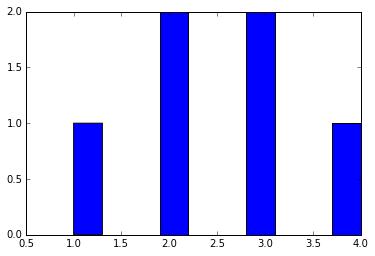
\includegraphics[width=.3\linewidth]{../../pictures/plthist}\hfill
	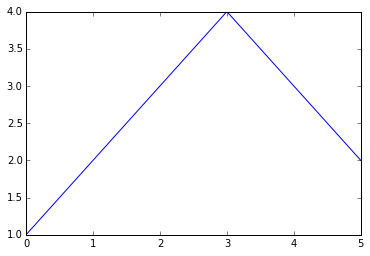
\includegraphics[width=.3\linewidth]{../../pictures/pltplot}\hfill
	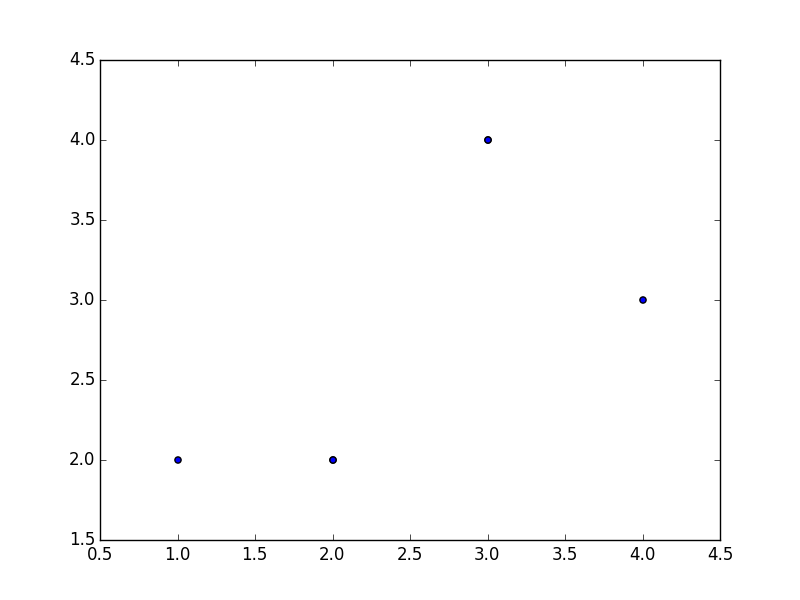
\includegraphics[width=.3\linewidth]{../../pictures/pltscatter}
	\caption{\label{fig:matplotlib}Examples of plots generated with \texttt{matplotlib}}
\end{figure}

\end{frame}





\section{Pandas}
\subsection{Working with dataframes}

\begin{frame}[plain]
	Pandas\\
	\textbf{Working with dataframes}
\end{frame}




\begin{frame}{When to use dataframes}
	\footnotesize
	\begin{columns}[t]
		\column{.5\textwidth}
		
		\begin{block}<1->{Native Python data structures (lists, dicts, generators)}
		pro:
		\begin{itemize}
			\item flexible (especially dicts!)
			\item fast
			\item straightforward and easy to understand
		\end{itemize}
		con:
		\begin{itemize}
			\item if your data is a table, modeling this as, e.g., lists of lists feels unintuitive
			\item very low-level: you need to do much stuff `by hand'
		\end{itemize}
		
		\end{block}
		
		\column{.5\textwidth}
		
		\begin{block}<2->{Pandas dataframes}
			pro:
			\begin{itemize}
				\item like an R dataframe or a STATA or SPSS dataset
				\item many convenience functions (descriptive statistics, plotting over time, grouping and subsetting, \ldots)
			\end{itemize}
			con:
			\begin{itemize}
				\item not always necessary (`overkill')
				\item if you deal with really large datasets, you don't want to load them fully into memory (which pandas does)
			\end{itemize}
			
		\end{block}
		
	\end{columns}
	
\end{frame}







\subsection{Plotting and calculating with Pandas}
\begin{frame}[plain]
	Pandas\\
	\textbf{Plotting and calculating with Pandas}
\end{frame}


\begin{frame}{}

More examples here: \url{https://github.com/damian0604/bdaca/blob/master/ipynb/basic_statistics.ipynb}
\end{frame}


\begin{frame}[fragile]{OLS regression in pandas}
\begin{lstlisting}
import pandas as pd
import statsmodels.formula.api as smf 

df = pd.DataFrame({'income': [10,20,30,40,50], 'age': [20, 30, 10, 40, 50], 'facebooklikes': [32, 234, 23, 23, 42523]})

# alternative: read from CSV file:
# df = pd.read_csv('mydata.csv')

myfittedregression = smf.ols(formula='income ~ age + facebooklikes', data=df).fit()
print(myfittedregression.summary())
\end{lstlisting}
	
\end{frame}


\begin{frame}[plain,fragile]{}

\begin{lstlistingoutputtiny}
OLS Regression Results                            
==============================================================================
Dep. Variable:                 income   R-squared:                       0.579
Model:                            OLS   Adj. R-squared:                  0.158
Method:                 Least Squares   F-statistic:                     1.375
Date:                Mon, 05 Mar 2018   Prob (F-statistic):              0.421
Time:                        18:07:29   Log-Likelihood:                -18.178
No. Observations:                   5   AIC:                             42.36
Df Residuals:                       2   BIC:                             41.19
Df Model:                           2                                         
Covariance Type:            nonrobust                                         
=================================================================================
coef    std err          t      P>|t|      [95.0% Conf. Int.]
---------------------------------------------------------------------------------
Intercept        14.9525     17.764      0.842      0.489       -61.481    91.386
age               0.4012      0.650      0.617      0.600        -2.394     3.197
facebooklikes     0.0004      0.001      0.650      0.583        -0.002     0.003
==============================================================================
Omnibus:                          nan   Durbin-Watson:                   1.061
Prob(Omnibus):                    nan   Jarque-Bera (JB):                0.498
Skew:                          -0.123   Prob(JB):                        0.780
Kurtosis:                       1.474   Cond. No.                     5.21e+04
==============================================================================

\end{lstlistingoutputtiny}
	
\end{frame}




\begin{frame}[fragile]{Other cool df operations}
\begin{description}
	\item[df{['age']}.plot()] to plot a column
	\item[df{['age']}.describe()] to get descriptive statistics 
	\item[df{['age']}.value\_counts()] to get a frequency table
\end{description}
and MUCH more
	
\end{frame}


\section{Exercise}
\begin{frame}[plain]
{\huge{Joanna will introduce you to the exercise} }
\vskip 1cm
... and of course you can also ask questions about the last weeks if you still have some!
\end{frame}


\end{document}


